\section{Discussion}
\label{sec:discussions}

%cfg: outline of some key points to be made in discussion

%What is the spin and orientation of  \sgra, the magnetic state of the near-horizon plasma (SANE, MAD, or something else?), the electron distribution function (in the standard models, what is $\Rh$?), the accretion rate, and the radiative efficiency?  We can't yet answer these questions with confidence because no model fully explains the data.

%Still, there are comprehensible trends in the model space that favor certain source parameters.  For black hole spin,

%- do the model tests constrain the source structure?
%    * inclination
%    * mad vs sane
%    * spin: no direct evidence in critical impact parameter size
%    common thread: higher temperature works better
%    * position angle is not constrained, as in imaging work.

%- many trends in measured values in the models.  Highlight a few themes that emerge:

%- possible explanations for large model variability

%- is there extended structure?

%- can we hide a $10^(38)$ erg/sec outflow in the galactic center?

%- alternative model studies are inconclusive on tilted and wind-fed models.  These models are live and need to be investigated with longer runs.

%- nonthermal models are also inconclusive, but signs are that the SED is the most important constraint here.  Some general factors affecting eDF.

%- importance of long duration runs

%- importance of better baseline coverage

%- bremsstrahlung and SANE models: possibly tighter constraints with more radially extended models.  Interesting to look at x-rays from ressler models.

%- \Mring image plane models likely to be inadequate with more data.  Already many of the images are poorly fit.  Need more

%- future analysis may be able to detect rotation

%- sigma cut matters for NIR.

%- about the statistical procedure used here

%- directions for future analysis.

%==============================================================================
\subsection{Origin of Variability Excess}

Most of our models have excess 230\GHz lightcurve variability compared to historical data.
Section \ref{sec:comparisons} mentions possible explanations for this, including extended flux and the possibility that our models are missing physical ingredients that would reduce their variability.

Recall that we characterize variability in the 230\GHz lightcurve through the distribution of the modulation index $\mi{3} \equiv \sigma/\mu$, where $\sigma$ is the standard deviation of the lightcurve and $\mu$ is the mean, in our case evaluated over a 3 hour interval.

It is possible that the origin of the variability excess lies in interpretation of the observations.
The observed $\mi{3}$ is, formally, only a lower limit.  Slowly varying, diffuse emission on larger angular scales could contribute to the observed mean flux ($\mu$) but not contribute to $\sigma$ and not be captured in models of the compact source.  Diffuse emission on scales larger than the VLBI images ($\sim 100\uas$) and smaller than connected element interferometer measurements ($\sim 100\,\mathrm{mas}$) is difficult to constrain.  The EHTC imaging strategy involves a self-calibration step that assumes no diffuse structure on scales between the zero-baseline and the shortest VLBI baselines (\citetalias{PaperIII}).  However, longer wavelength VLBI observations place fairly significant constraints on any emission on these scales under the assumption of flat or steep spectra.  For instance, 1.3 and 7\mm VLBI observations that use the Los Alamos-Pie Town-VLA baselines probe scales of $\sim 1$ to $10\,\mathrm{mas}$ and demonstrate no inconsistency in closure amplitudes and closure phases with a symmetric, two-dimensional Gaussian model \citep{2004Sci...304..704B}.  VLBI observations at 3mm wavelength are also fully consistent with a two-dimensional Gaussian model with an upper limit of $\sim 10\,\mathrm{mJy}$, or approximately 1\% of the total flux density \citep{2019A&A...621A.119B}.  Additionally, a dust contribution is constrained by shorter wavelength ALMA observations that find a flat or slightly falling spectrum up to 900 GHz \citep{2019ApJ...881L...2B}.  A significant diffuse dust contribution would only be consistent if its properties were tuned to match a steeply falling compact synchrotron spectrum, which would likely be inconsistent with the significantly variable far infrared component of \sgra emission \citep{2016ApJ...825...32S, 2018ApJ...862..129V}.

Future observations with denser, short-baseline coverage such as that provided by the Kitt Peak to SMT baseline will enable tighter constraints on any diffuse component.  If confirmed, the presence of diffuse flux would require re-normalization of the models and re-evaluation of the constraints.  An adjustment of $\sim 30\%$ in the compact flux would bring most MAD models into compliance with the $\mi{3}$ constraint; since $F_{230} \sim \dot{M}^2$ this would require only a $15\%$ change in model normalization.  We speculate that this would have only a modest effect on model constraints.

The variability excess might also be a failure in the models.  Two physical effects top our list of suspects: collisionless effects and cooling.

We have modeled the accreting plasma as an ideal fluid (short mean free path approximation) when in fact it is collisionless, with Coulomb mean free path large compared to $\rg$.  This is less worrisome than one might think: electrons and ions are confined to helical orbits around field lines, implying an effective mean free path perpendicular to the field lines given by the gyroradius $\sim 56 \Theta_e [B/(30\,\mathrm{G})]^{-1} \cm \ll \rg$.  The mean free path parallel to field lines is still long, but may be limited by scattering off plasma fluctuations excited by kinetic instabilities.

A relativistic fluid model based on this notion has been developed by \citet{2015ApJ...810..162C} and studied numerically by \citet{2017MNRAS.470.2240F}.  The leading order corrections to the ideal GRMHD are conduction and pressure anisotropy (i.e., viscosity).  It is not known what the effect on $\mi{3}$ might be, but numerical integrations suggest the effect on turbulent magnetic stresses in MAD models is weaker than SANE models \citep{2017MNRAS.470.2240F}. In the future global kinetic general relativistic particle-in-cell simulations can test how well this model describes collisionless accretion flows.

Our models also neglect cooling.  Cooling is likely to be most important where the electron temperature is highest. The electron temperature is expected to fluctuate, so cooling may round off the peaks in the lightcurve when those are produced in localized heating events where cooling times are short.  To investigate cooling self-consistently requires integration of an electron energy equation, as in \cite{2015MNRAS.454.1848R}, and that requires a model for partitioning dissipation between the electrons and ions, as well as---to capture radiative cooling---assignment of a density scale (mass unit or accretion rate) at the time the GRMHD model is run.  This requires iterative analysis of these model sets, which is beyond the scope of this paper.  We note that we have analyzed $\mi{3}$ in a set of models with self-consistent electron heating and without radiative cooling; these models still show a variability excess.

There are more prosaic possible explanations for the variability excess: numerical inaccuracies in radiative transfer, truncation error in the GRMHD integrations (limited resolution), limited simulation duration, or misspecification of the adiabatic index.  These are considered in Appendix~\ref{app:numerical}.  There is no evidence that any of these effects produces a significant correction to $\mi{3}$.

One plausible scenario is that each of the above effects (extended flux, viscosity, and cooling) contributes 10\% toward moving $\mi{3}$ from the models and data closer together. A small correction to $\mi{3}$ from numerical resolution in ideal GRMHD models also cannot be ruled out.



\subsection{Accretion Rate and Outflow Power}
\label{sec:accrate_outflowpower}
% this subsection should go first because it is important for discussion that follows.

% cfg checked 14 dec
% \monika{this section has been revised, please check and revise further}

% figures go first to align them with text better
% these plots should be shown together because they share rhigh label, so I merged them

\begin{figure*}
  \centering
  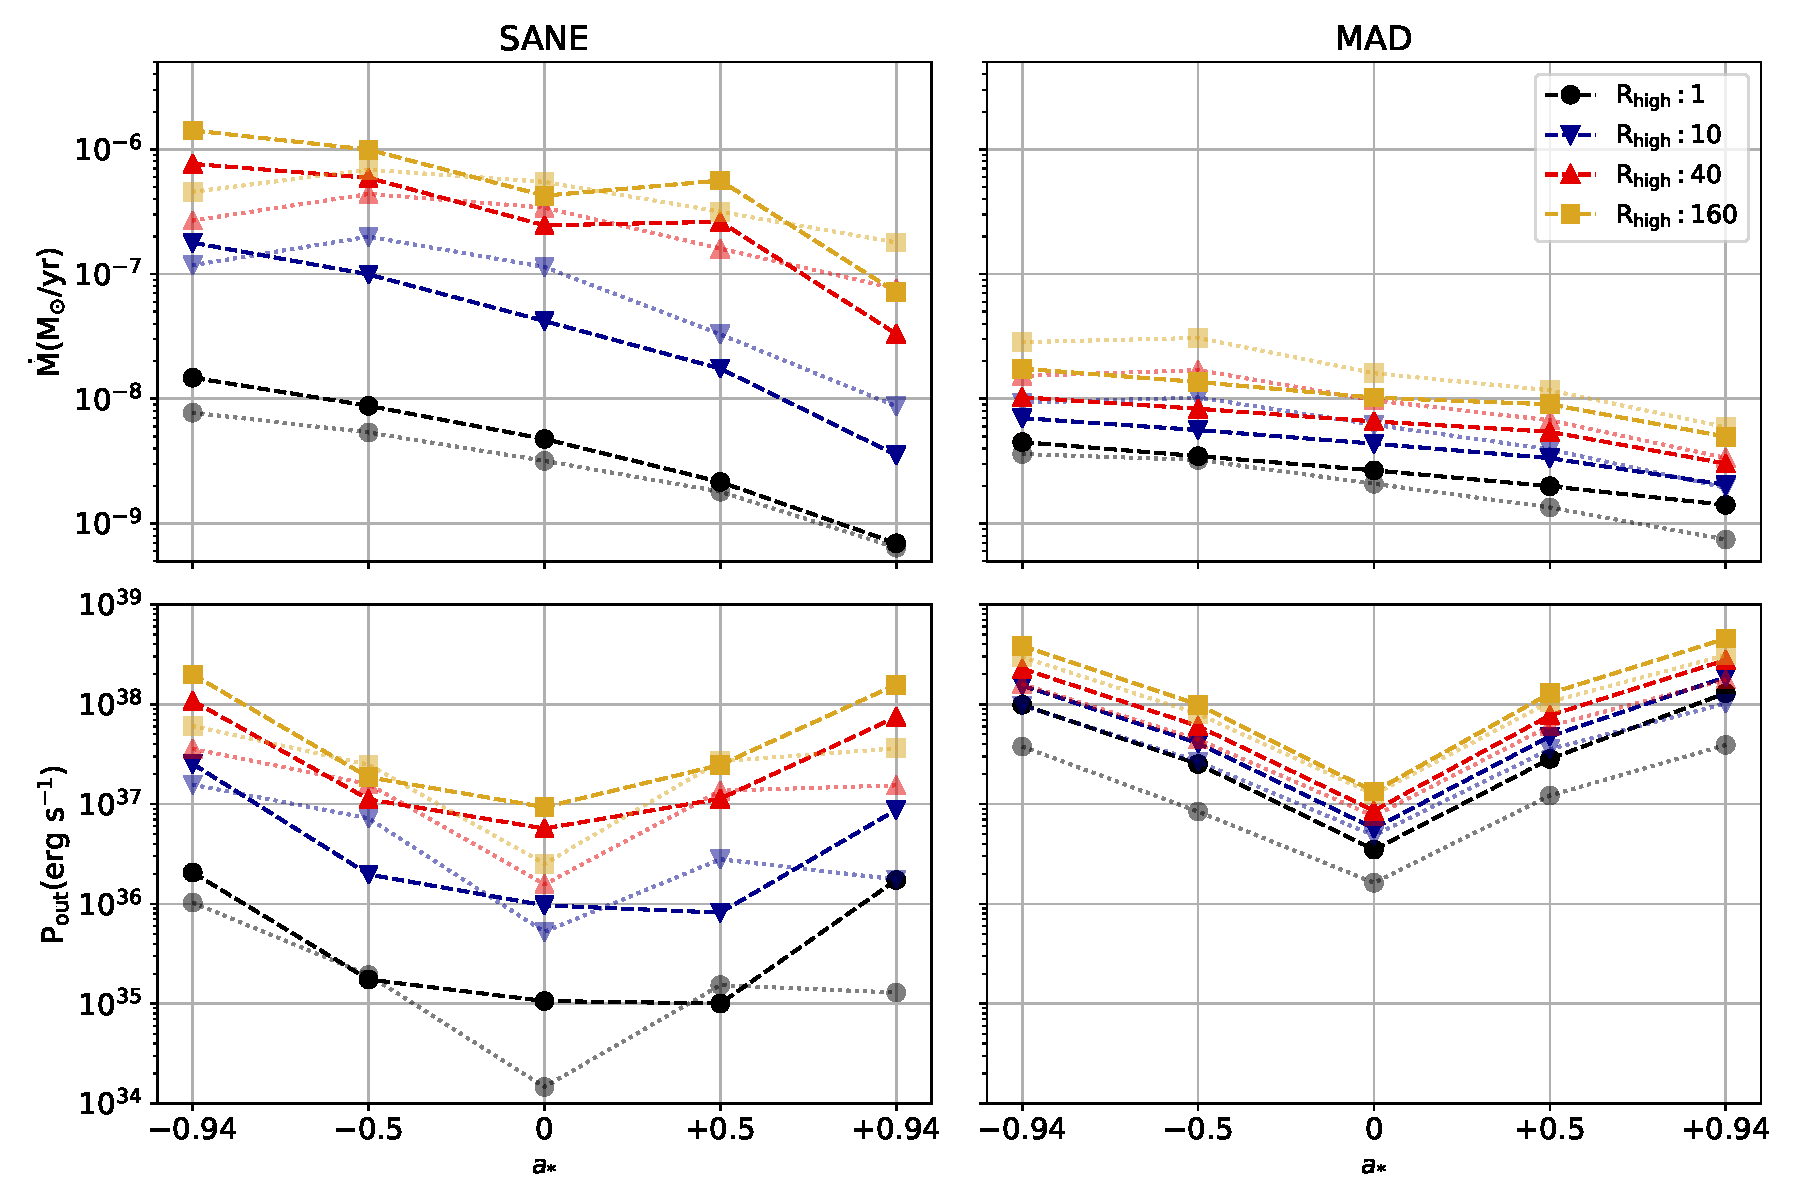
\includegraphics[width=0.95\textwidth]{figures/bhac_kharma_average_mdot_pout.pdf}
  \caption{{\it Top:} Accretion rate $\dot{M}$ for standard models. Since $\dot{M}$ depends weakly on inclination $i$, we show only $i=50\degree$. {\it Bottom:} Outflow power $P_\mathrm{out}$ for standard models at $i = 50\degree$. The colors and markers vary with $\Rh$. The dashed lines correspond to \kharma thermal models while the dotted lines indicate \bhac thermal models.}
  \label{fig:accretion_outflow_power_illinois_thermal}
\end{figure*}

% \begin{figure*}
% \centering
% 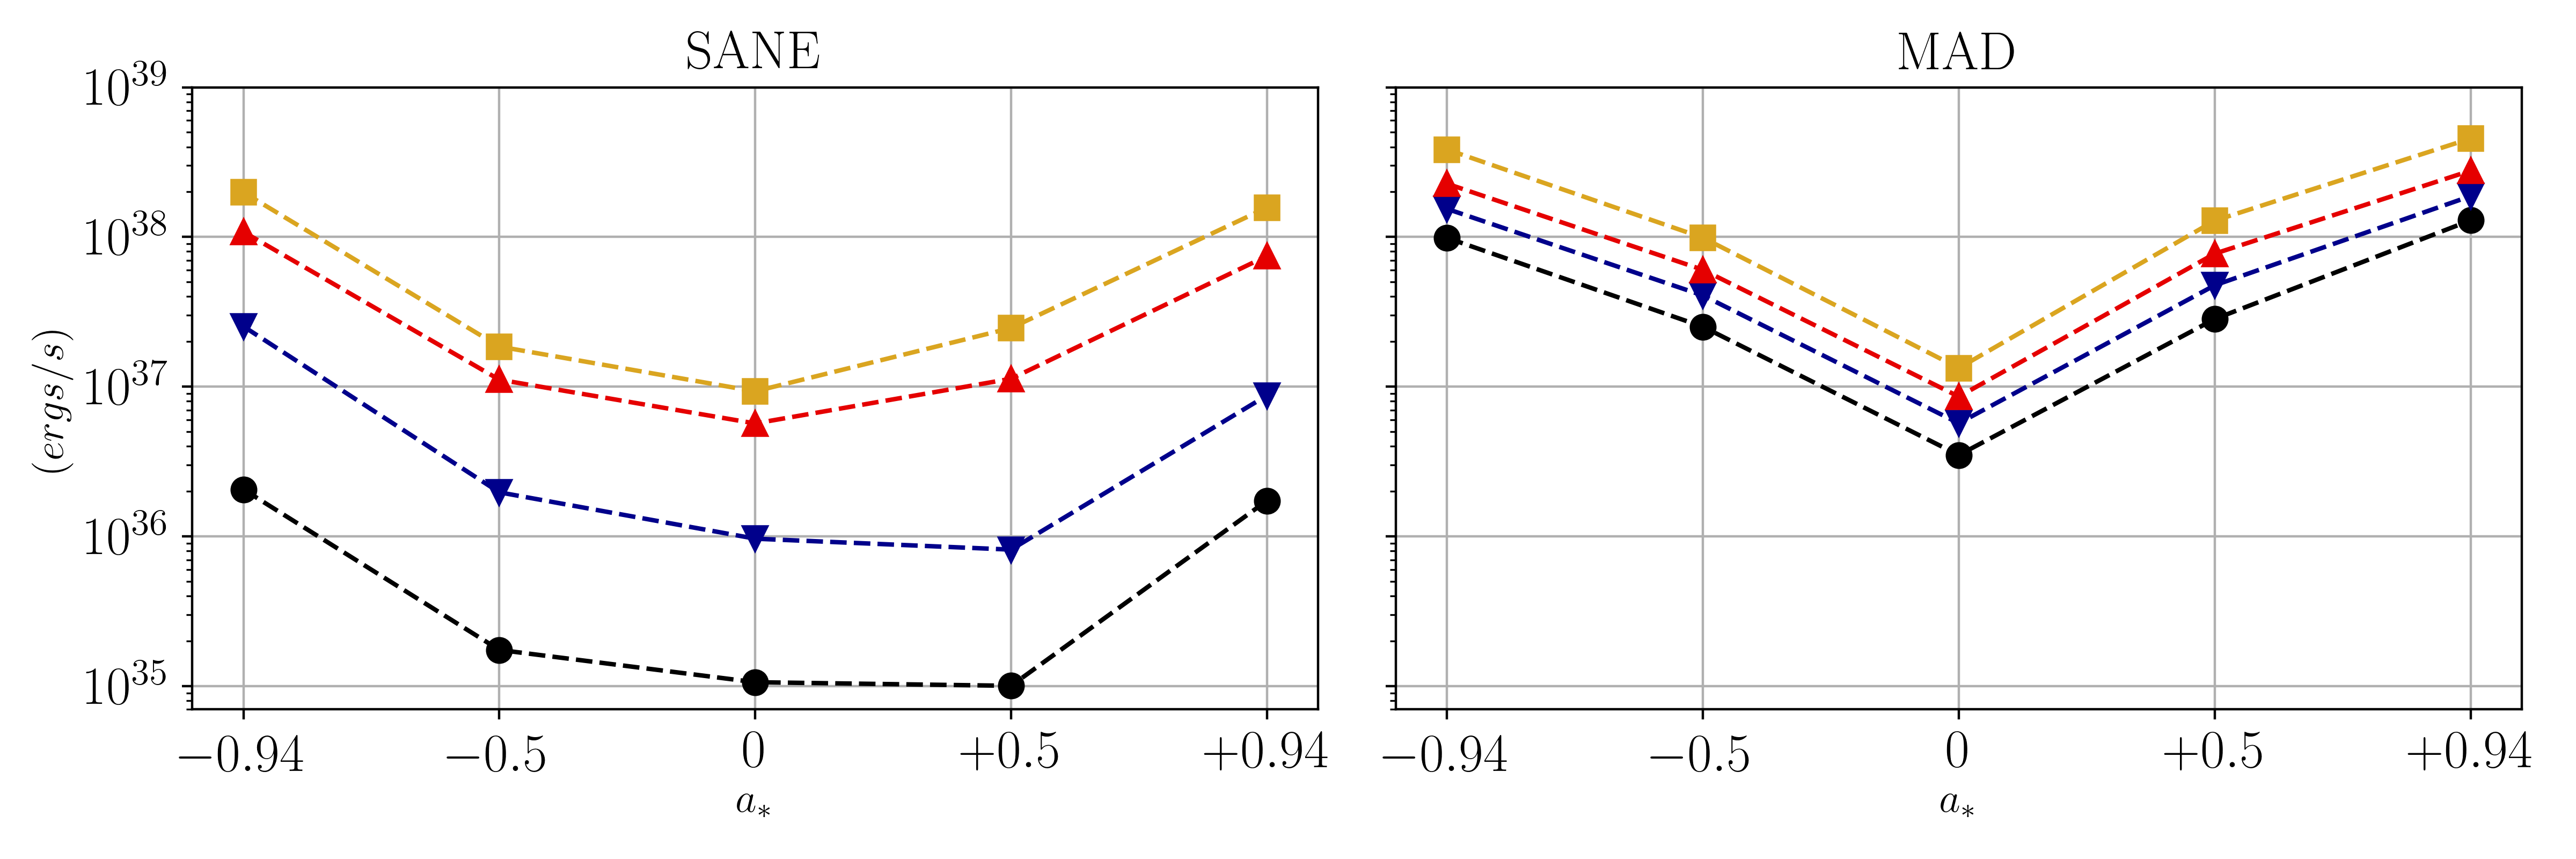
\includegraphics[width=0.95\textwidth]{figures/illinoisv3_average_outflow_power.png}
% \caption{Outflow powers measured in \kharma thermal models at an observer inclination $i=50^{\circ}$. The colors and markers are the same as \ref{fig:accretion_illinois_thermal}.}
% \label{fig:outflow_illinois_thermal}
% \end{figure*}

What is the accretion rate in \sgra?  In our models, we measure the time-averaged accretion rate
%\cmf{Hector is working on the results from the BHAC runs including non-thermal emission models, should be done over the weekend}
\begin{equation}
  \dot{M} = \frac{1}{\Delta t}\int dt\int d\theta d\phi\hspace{0.1cm}\sqrt{-g}\big(-\rho u^{r}\big),
\end{equation}
at the event horizon; the quantity in the parenthesis is the inward rest-mass flux.

Figure~\ref{fig:accretion_outflow_power_illinois_thermal} (top panels) shows the time-averaged $\dot{M}$ (in solar masses per year) for the \kharma and \bhac thermal models.  The accretion rates follow immediately once the models are normalized so that $\langle F_{230}\rangle = 2.4\,\mathrm{Jy}$.  A listing of $\dot{M}$ for all models for which it is available is provided in Appendix \ref{app:tables}.

% cfg original version
%MAD models accrete at $10^{-9}$ to $10^{-8} M_{\odot}\yr^{-1}$; SANE models have a broader range, $10^{-9}$ to $10^{-6} M_{\odot}\yr^{-1}$.  For all models $\partial\dot{M}/\partial\Rh > 0$.  This can be understood as a consequence of three facts: \emph{i}) thermal synchrotron emissivity is an increasing function of temperature; \emph{ii}) where $\beta > 1$ the electron temperature $\propto \Rh^{-1}$; \emph{iii}) in MAD models a relatively small fraction of the emitting plasma lies at $\beta > 1$ (cf.~Figure~4 in \citetalias{M87PaperV}).  It follows that $\partial\dot{M}/\partial\Rh > 0$ is required to maintain $F_{230} = 2.4\,\mathrm{Jy}$, with a steeper derivative for SANE models where the emissivity of more electrons is reduced by increases in $\Rh$.  For both SANE and MAD $\partial\dot{M}/\partial\abh < 0$.  This follows from the dependence of temperature on spin shown in Figure~\ref{fig:grmhd_temp}: higher spin corresponds to higher temperature.

% new vedant version
The MAD models accrete at $10^{-9}$ to $10^{-8} M_{\odot}$yr$^{-1}$ while the SANE models have a broader range, $10^{-9}$ to $10^{-6} M_{\odot}$yr$^{-1}$. $\dot{M}$ is an increasing function of $\Rh$. This can be understood as a consequence of three facts: (a) the thermal synchrotron emissivity is an increasing function of temperature; (b) the electron temperature is inversely proportional to $\Rh$; (c) the models need to normalized so that $\langle F_{230}\rangle$ $=$ 2.4Jy. The SANE models exhibit a stronger dependence on $\Rh$. The emission in the SANE models is predominantly from regions with large $\beta$, where the electron temperature is regulated by $\Rh$. MAD models produce a significant fraction of the emission in regions with $\beta\sim 1$, where $\Rh$ does not notably influence electron temperature and thus have a weaker dependence on $\Rh$ (cite figure 4 in M87 paper V). For both SANE and MAD models, $\dot{M}$ reduces with spin. This follows from the dependence of temperature on spin shown in Figure 2: higher spin corresponds to higher temperatures

Retrograde SANE, $\Rh=40$ and $160$ models produce the largest accretion rates, $\dot{M} \sim 10^{-6}M_{\odot}\yr^{-1}$.  These models have a high midplane density of cool electrons that overproduce x-ray emission through bremsstrahlung and are therefore ruled out.   Our critical beta models have accretion rates that lie between the standard model values for $\Rh = 10$ and $\Rh = 40$ for the selected critical beta parameter values ($f=0.5$, $\beta_\mathrm{crit}=1$).

%, so $F_{230}$ is less sensitive to $\Rh$ in MADs.  (ii) $d\dot{M}/d\Rh > 0$. Since electron temperature at $\propto \Rh^{-1}$ where $\beta > 1$, larger $\Rh$ implies cooler electrons so to maintain an average flux density of 2.4\,Jy at 1.3\mm, the corresponding $\mathcal{M}$ increases. (iii) SANE models exhibit a more pronounced change in $\dot{M}$ with changes in $\Rh$ as compared to the MAD models. The emission in the SANE models is predominantly from regions with large plasma $\beta$, where the electron temperature is regulated by $\Rh$; MAD models produce a significant fraction of the emission in regions with $\beta\sim 1$, where $\Rh$ does not notably influence electron temperature (cf. Figure~4 in \citetalias{M87PaperV}). (iv) The retrograde, SANE, $\Rh=40$ and $160$ models produce the largest accretion rates, $\dot{M}\sim 10^{-6}M_{\odot}$yr$^{-1}$. However, these models are ruled out due to overproduction of x-ray emission. (v) The thermal models with the critical-$\beta$ electron temperature assignment scheme predict accretion rates that lie between the $\Rh=10$ and 40 values for the chosen set of parameters ($f=0.5$, $\beta_\mathrm{crit}=1$).

%\color{red}{\bf please add if bhac confirms this general trends. add figure but it would be best to plot this all together using maybe more transparent lines for bhac sims in the existing figure.}
%\color{black}

How do our $\dot{M}$ compare with earlier estimates?  Linear polarization and Faraday rotation measurements at millimeter and sub-millimeter wavelengths \citep{2000ApJ...538L.121A, 2000ApJ...545..842Q, 2003ApJ...588..331B, 2006ApJ...640..308M, 2006JPhCS..54..354M, 2006ApJ...646L.111M} and x-ray emission \citep{2003ApJ...591..891B, doi:10.1126/science.1240755} combined  with semi-analytic models predict $\dot{M} \sim 10^{-9} - 10^{-7} M_{\odot}\yr^{-1}$.  The broad range of values is due to the differences in regions of radio emission in the theoretical models that are considered (ADAFs: \citealt{1998ApJ...492..554N, Yuan_2003}; Jet models: \citealt{1993A&A...278L...1F, 2000A&A...362..113F}; ADAF+jet models: \citealt{2002A&A...383..854Y}).  All our MAD $\dot{M}$ fall within the range of these historical observational estimates. Interestingly almost all SANE models with larger $\rhigh$ parameter (except SANE $\abh=0.94$, which is one of our best models) have $\dot{M}$s that are inconsistent with earlier estimates.

%\color{red}
%{\bf LEFT OVER COMMENT TO INCORPORATE: Models at the highest accretion rate are ruled out by overproduction of x-ray emission.  If our models were in equilibrium over a larger range in radius, bremss from larger radius might increase the x-ray flux and disfavor more models.}
%\color{black}

All our standard models produce outflows in the polar regions.  In many cases the outflows can be divided into a slower, denser disk wind and a relativistic, high $\sigma$ Poynting jet.  The outflows have a power that is comparable to or larger than the bolometric luminosity.  What is the outflow power $P_\mathrm{out}$?

%Our numerical simulations of black hole accretion in \sgra consistently produce relativistic outflows in the polar regions (in the standard models these outflows can be divided into disk wind/corona and relativistic jet that is often strongly magnetized and nearly hollow). These relativistic outflows have an electromagnetic energy that is typically comparable or larger than the bolometric luminosity of \sgra. We are interested in the outflow power to predict if an outflow can be observed e.g., at larger distances from the black hole where the outflow energy gets dissipated.

First we must define $P_\mathrm{out}$.  There are a number of competing definitions in the literature: \citet{refId0}, \citet{2014A&A...570A...7M} cut on  Bernoulli parameter Be, while \citet{10.1111/j.1365-2966.2012.22002.x} consider the ratio of energy flux to rest mass flux $\mu$, and \citetalias{M87PaperV} applies a $\beta\gamma$ cut to define $P_\mathrm{out}$.  Here we use the time-averaged outflow power near the poles \citetalias{M87PaperV}:
\begin{equation}
  P_\mathrm{out} \equiv \frac{1}{\Delta t}\int dt \int d\phi \int_\mathrm{poles} d\theta \sqrt{-g}\left(-T^{r}_{t}-\rho u^{r}\right),
\end{equation}
where ``poles'' means $\theta < 1\,\mathrm{rad}$ or $\theta > (\pi-1)\,\mathrm{rad}$ at $\theta$ where the time- and azimuth-averaged energy flux is outward.  The integral is evaluated at $r = 100\rg$. $P_\mathrm{out}$ includes power in the relativistic Poynting jet, if present, and in the slower, denser disk wind.

%In Figure~\ref{fig:outflow_illinois_thermal}
In Figure~\ref{fig:accretion_outflow_power_illinois_thermal}
(bottom panels) we compute $P_\mathrm{out}$ for the standard models. As expected, the outflow power increases with the magnitude of black hole spin. SANE models have $P_{out}$ in the range ~$10^{35} \ergps$ to $10^{38} \ergps$. Evidently $P_{out}$ increases with $\Rh$,  reflecting the behaviour of $\dot{M}$: higher $\dot{M}$ models have stronger magnetic fields. MAD models have $P_\mathrm{out}$ in the range $10^{37}$--$10^{39} \ergps$ and are, on average, larger and less sensitive to $\Rh$, again reflecting the behavior of $\dot{M}$.
% 14-dec: yes, need statement about nonthermal models.
%\color{red}{\bf please add results from bhac for comparison if they are available.}\color{black}
%\color{red}{\bf one should say a few words how electron distribution function changes mass accretion rate estimates and jet powers.}\color{black}

Many high spin or large $\Rh$ models have $P_\mathrm{out} \sim 10^{38} \ergps$.
An outflow with this power could produce dramatic observable effects in the dense interstellar medium of the Galactic Center.  For instance, the x-ray transient CXOGC J174540.0-290031, located only 0.1\pc from \sgra and with an estimated jet power of $\sim 10^{36}\ergps$ produced a compact bipolar lobe at radio wavelengths with peak flux densities near 100$\,\mathrm{mJy}$ \citep{2005ApJ...633..218B}.  A more continuous  outflow, however, might clear out a significant volume of space, making identification of any interaction with the ISM less certain.  Nevertheless, there have been a number of large scale features that have been suggested as the result of interaction of a jet with the ISM \citep[e.g.,][]{2013ApJ...779..154L,2021ApJ...922..254C}.

% cfg 14 dec: revised into par above following contribution from geoff.
%Following \citet{2007MNRAS.379.1519M} one may ask: is it possible to hide such powerful outflow in the Galactic Center? Unlike for \m87, there is no observational estimate for power of a putative jet in \sgra system. There have been several studies at radio, x-ray and $\gamma$-ray that have suggested the presence of a mildly relativistic outflow based on morphological structures observed in the \sgra complex (\citealt{2012ApJ...758L..11Y,2012AAS...22051303S,Li_2013,2019ApJ...875...44Z,2021arXiv210713402B} and references therein). However, due to the low luminosity of \sgra and the presence of the interstellar scattering screen (\citealt{2016ApJ...824...40O,2017MNRAS.471.3563D,2018ApJ...865..104J,2019A&A...621A.119B}) there is no direct evidence of the jet or outflow from \sgra. %\monika{EHT data interpretation suggest that we cannot exclude the presence of an outflow.???}

%==============================================================================
\subsection{Electron Distribution Function}

One of the central uncertainties in modeling \sgra is how to assign the electron distribution function (eDF).  Do the surviving models have anything to say about the eDF?

In our standard models, thermal eDFs with equal ion and electron temperature ($\Rh = 1$) are ruled out, in most cases by more than one constraint.  For MAD models this is easily explained: Comptonization is strong at $\Rh = 1$ and x-rays are overproduced.  The electron temperature is a maximum when $\Rh = 1$, if all other parameters are fixed. For MAD models, $\dot{M}$ and therefore the electron scattering optical depth $\tau_\mathrm{es}$ is insensitive to $\Rh$.  Since the amplitude of the first Compton bump is $\propto y = 16 \Theta_e^2 \tau_\mathrm{es}$, the high $\Theta_e$ at $\Rh = 1$ produces a large x-ray flux.  For SANE models the situation is more complicated (see Appendix~\ref{app:tables}), with an \mring width rejecting many $\Rh = 1$ models at $\abh \le 0$, and 86~GHz flux and size rejecting the rest.  The latter is a consequence of model electron temperature reaching a maximum at large $\abh$ and low $\Rh$, so that optical depth is minimum and therefore so is the 86~GHz image size.

In standard SANE models the sense of the x-ray constraint is reversed: bremsstrahlung is strong and x-rays are overproduced where $\Rh$ is {\em large}.  Again this is easily understood: when $\Rh$ is large the midplane electrons are cold, the accretion rates (and therefore $n^2$) are high, and the bremsstrahlung emissivity is large.  More generally the x-rays provide a strong constraint on the presence of dark (subrelativistic) electrons, which are otherwise undetectable in millimeter wavelength emission or absorption, although they can produce strong Faraday rotation.

We have also tested a large set of nonthermal models, which have a power-law tail on the eDF.  Although integration times for the nonthermal models are too short to provide strong model constraints, there are trends that emerge from the existing data.

First, the 230~GHz images are relatively insensitive to the presence of nonthermal electrons, at least for the nonthermal electron models we have studied here.  This is encouraging: the 230~GHz image is generated by electrons in an approximately thermal core of the eDF, and is relatively insensitive to the behavior of the tails.

Second, as one might expect, the 2.2\um flux density is a strictly increasing function of nonthermal electron density.  In many models (e.g. the variable efficiency models of Section 4.2.3) the addition of a power-law tail changes a thermal model that passes the NIR test into a nonthermal model that fails.

Third, it is important to understand that many of the nonthermal models we use are linked to the $\Rh$ prescription in some way.  For example, the kappa distribution function contains a width parameter $w$, and this is set using an $\Rh$-like prescription with width depending on $\beta$.  Our nonthermal models are only a few points in a vast function space of possible nonthermal parameterizations, with none of the models considered allowing for an electron energy density that depends on plasma history as well as instantaneous plasma state.


%==============================================================================
%\subsection{Inclination}

%\note{Michi to provide first draft}
%\note{Strong constraints on inclination from \mring fitting.}
%\ckc{ck's first pass}

%When the accretion flow around a black hole has enough angular momentum, the corresponding black hole image is sensitive to its inclination---in an edge-on case, the image is more asymmetric, with one side lighted up because of Doppler boosting; for a face-on case, the image is a more symmetric ring.
%\gw{I agree with the preceding, but I'm worried that this may be misleading with respect to how the geometry of the spacetime influences the image. For example, even if the flow angular momentum is zero, if bhspin > 0, then the corresponding image is *still* sensitive to inclination.}
%\ckc{Good point.  Feel free to edit.}
%However, this dependency is weak in a low angular moment accretion flow, or when frame dragging cancels out the Doppler effect. These situations include the MAD state, where the accretion flow is magnetically supported, and retrograde accretion flows \citep{2021arXiv210503424M}.

%The above conditional dependency of the asymmetry of the ring and
%inclination makes it non-trivial to measure inclination from the
%observation.
%In addition, it is important to note that the asymmetry described
%above does not directly corresponds to the \mring asymmetry.
%Consider a situation that the Doppler boosting is so extreme that only
%the bright side of the photon ring is visible, while the dim side is
%hidden under the noise.
%In such a situation, the \mring (or the g\mring in \citetalias{PaperIV})
%may misidentify the boosted side as the full image, and return a low
%asymmetry, small image size, and wide image width.
%This is the reason that it is difficult to directly link one \mring
%measurement to the inclination.
%Nevertheless, given that the EHT observation is surprisingly
%symmetric, the \mring asymmetry measurement is not constraining.
%In stead, the \mring size disfavors the face-on images.

%==============================================================================
%\subsection{Position Angle}

%\note{Virtually no constraint on position angle [check \mring fits]}

%According to the data, the image of \sgra is surprisingly symmetric.
%The position angle measurement is dominated by noise.
%Our visibility domain constraining is therefore not constrianing on
%the position angle.

%==============================================================================
%\subsection{Black Hole Spin}

%\note{Still quite weak constraints on black hole spin.}

%Given that the size and the shape of the black hole shadow is
%insensitive to its spin, the black hole spin remains one of the most
%difficult black hole parameters to constraint.

%However, as we discussed earlier, the asymmetry of the image does
%depend on the black hole spin, assuming that there is significant
%angular momentum in the accretion flow, In this sense, the
%astrophysics can help us narrow down the spin.
%Specifically, the \mring diameter disfavors low spin models.
%However, with the current u uncertainties in, e.g., the eDF, we are
%not be able to report an acutal spin measurement.


%==============================================================================
\subsection{Caveats and Limitations}\label{sec:limits}

%%%%%%%%%%%%%%%%%%%%%%%%%%%%%%%%%%
% \note{to be discussed: how much we would like to discuss polarization emission?}\textcolor{red}{RJA: We should mention the M87 Polarization Collaboration papers \cite{M87PaperVII}, including a comparison of whether Sgr A* is similar enough (e.g., MAD with vertical fields Faraday depolarized on much of the accretion flow) to have an azimuthally spiral EVPA pattern. Figures in  \citep{Emami2021} have similar morphology}.

% \hyp{to-do :  adding historical RIAF fitting result to proto-EHT observations; how recent  GRMHD simulation and subsequent GRRT post-processing suggest other key parameters onto the Broderick 2005 RIAF model; jet componenet? cross referencing MCFE RIAF analysis product?} A proto-EHT array described in \cite{Doeleman2008} estimated the Sgr A* emitting region profile as a circular Gaussian with intrinsic size $37^{+16}_{-10}\ \mu$as.

% % EHT flux vs. baseline observations constrain the emitting region intrinsic size to 37 microarcseconds for a circular Gaussian emission profile

% More recent measurements of closure phases of a few degrees \cite{Fish2016} suggest an asymmetric ring-like profile, with major axis 56 microarcseconds
%%%%%%%%%%%%%%%%%%%%%%%%%%%%%%%%%%

%------------------------------------------------------------------------------
\subsubsection{Collisionless plasma effects}

%\monika{some of the collisionless aspects are addressed in appendix C1 in subsection on selfconsistent electron heating models. check if this is mentioned below}
%\br{I rewrote a little bit and added a sentence.}

{The mean free path to Coulomb scattering for particles is typically larger than or comparable to the system size in \sgra, rendering its plasma collisionless. The GRMHD models employed in this work describe a collisional system, whereas a first-principles modeling of the collisionless plasma requires a fully kinetic treatment. General relativistic (radiative) kinetic simulations are crucial for dynamically probing the electron temperature, effects of non-thermal distribution functions, and pressure anisotropy and their interplay with radiation in collisionless plasma in the accretion disk and jet. While global general relativistic kinetic simulations cannot be performed with full physical separation between microscopic plasma scales (the particle's Larmor radius $r_{\rm L}$, and plasma skin depth $d_{\rm e}$) and macroscopic scales (the gravitational radius $r_{\rm g}$), they can achieve the right hierarchy of scales ($r_{\rm g} \gg d_{\rm e} \gg r_{\rm L}$) for magnetized plasmas \citep{2018A&A...616A.184L,2018ApJ...863L..31C,2019PhRvL.122c5101P,2020PhRvL.124n5101C,2020ApJ...895..121C,2020ApJ...902...80K,2021A&A...650A.163C,2021PhRvL.127e5101B}. Even in GRMHD, it is computationally challenging to resolve plasma heating processes powering the observed radiation in a converged manner. It is currently not yet feasible to resolve dissipation at the smallest scales of the turbulent cascade or the interplay between turbulence and reconnection at a similar level as in local box simulations \citep{2012ApJ...755...50R,2013ApJ...773..118H,2015PhRvL.114f1101H,2016PhRvL.117w5101K,2017PhRvL.118e5103Z,2018PhRvL.121y5101C,2018ApJ...859..149I,2019PhRvL.122e5101Z,2021ApJ...921...87N,2021arXiv211108188C}. However, \citet{2019ApJS..243...26P} and \citet[in prep.]{Olivares_et_al} show that the global accretion dynamics (mass accretion rate, magnetic flux on the horizon, and MRI quality factor) are converging between the different simulations in this work. Kinetic processes in the (near-)collisionless plasma may increase the effective particle collision rate \citep[see, e.g.,][]{2016PhRvL.117w5101K}. Deviations from the infinitely conductive ideal fluid approximation may alter the thermodynamics of the flow \citep[see, e.g., ][and Appendix C1]{2017MNRAS.470.2240F}. Some aspects of (near-)collisionless plasma dynamics can be described with non-ideal effects (e.g., viscosity, resistivity, heat conduction, pressure anisotropy) in GRMHD models for black hole accretion, e.g.,  \cite{2014MNRAS.440L..41B,2015ApJ...810..162C,2016MNRAS.456.1332F,2017ApJ...837...92C,2017MNRAS.470.2240F,2018ApJ...859...28Q,2019ApJS..244...10R,2019ApJ...882....2V,2020ApJ...900..100R,2021PhRvD.104j3028M,2021arXiv211103689N,2021arXiv211105752M}. For example, the first efforts have recently been made with high-resolution global GRMHD simulations to capture heating through magnetic reconnection in the largest current sheets in the system \citep{2020MNRAS.495.1549N,2020ApJ...900..100R,2021MNRAS.508.1241C,2021arXiv210915115R,2021arXiv211103689N}.}

%------------------------------------------------------------------------------
\subsubsection{Positrons}\label{sec:pair}

% cfg 14 dec: edited and marked comments as resolved
%\monika{i think this section should start with some general statement why do we want to consider positrons at all.}
%\ckc{I refer to this section from the eDF section.  Please feel free to move this around as long as we keep the label.}

%\monika{Also, is it possible to incorporate this positron story into Caveats and Limitations?}
%\br{I would add it as a subsection (with a subtitle) of the caveats, and it indeed needs a general statement why we want to consider positrons (I would mention magnetosphere (or potential jet that we dont see?) is pair plasma, and (non-thermal) positrons (accelerated in a gap, or by a current sheet in the jet/magnetosphere) can be mixed into the disk through reconnection or instabilities at the jet base, injecting non-thermal magnetized blobs into the disk}\monika{arent most of the collisionless kinetic plasma simulations you report above actually done for electron-positron plasmas? i think this should be maybe connected somehow}\br{I would not mix those paragraphs but do it as you did now (with separate subtitles), because the main point the two paragraphs are making is different (I think the current subtitles reflect that well). We could indeed connect an introducing sentence of this positron paragraph to the collisionless paragraph:}


%\br{``
%The black hole magnetosphere or potential jet region may consist mainly of highly magnetized electron-positron pair plasma produced by pair discharges. The pair plasma can be accelerated to non-thermal power-law energy distributions in spark gaps or reconnecting current sheets \citep{2018A&A...616A.184L,2018ApJ...863L..31C,2019PhRvL.122c5101P,2020PhRvL.124n5101C,2020ApJ...895..121C,2020ApJ...902...80K,2021PhRvL.127e5101B} and potentially get mixed into the accretion disk through the exhaust of the reconnection layer \citep{2021arXiv210915115R}.
%''}

So far we have considered only ion-electron plasmas, but pairs can be produced in the 230 GHz emission region through pair discharges or through so-called pair drizzle.  How might our neglect of pairs affect the models?

The importance of pairs has been assessed using phenomenological models \citep{2020ApJ...896...30A, 2021arXiv210105327E} and depends sensitively on the efficiency with which a reservoir of magnetic energy can be converted into pairs.  If this efficiency is large then pairs can significantly increase intensity in the jet region.

Production of pairs through the drizzle process is weak in \sgra because its luminosity is so low.  \cite[][see also \citealt{2021ApJ...907...73W}]{2011ApJ...735....9M} estimate the drizzle pair density of \sgra to be $10^{-8}\cm^{-3}$.  This is well below the Goldreich-Julian density $\sim \abh B c^2/(4 \pi e G M) \sim 10^{-2} \abh [B/(30 {\rm G})] \cm^{-3}$ required to screen electric fields, suggesting pair discharges are likely.  If pair discharges serve only to raise the pair density to the Goldreich-Julian density, however, then the jet is unlikely to outshine the accretion flow, where the magnetic field strength is similar to that in the jet but the characteristic number density is $\sim 10^6 \cm^{-3}$.  The maximum conceivable impact of pairs on EHT observations is obtained by converting about half of the magnetic energy density into pairs with Lorentz factor $\sim 30$ so that in \sgra's $\sim 30$G magnetic field the emissivity of the resulting pairs peaks close to 230\GHz.  Then the pair density $\sim 10^{6} \cm^{-3}$ and the jet might compete with the accretion flow.


%\cite{2006MNRAS.367..905B} devised a canonical model of Sgr A* as a  radiatively inefficient accretion flow (RIAF). Semi-analytic RIAF models implementing  this using the general relativistic ray tracer GRTRANS \citep{2016MNRAS.462..115D} can be found in  \cite{2021arXiv210105327E}, where  positrons are included using emission modeling motivated in  \cite{2020ApJ...896...30A}. The Figs. 1-3 %\ref{fig:EmamiRIAF}
%models from \cite{2021arXiv210105327E} shows Stokes maps and polarized spectra of a \cite{2006MNRAS.367..905B} RIAF with plasma $\beta=10$ and 1$\%$ of the emitting particles nonthermal electrons. The near-extremal ($a/M=0.998$) model shown exhibits Doppler boosting asymmetry in a crescent-shaped intensity pattern with a spiral global electric vector polarization angle (EVPA) pattern and polarization preferentially distributed within this region.

%\hyp{As phenomenological models are not considered in this work, the position effect in this subsection may rewrite in a way only focus on the resulting effects and its possible impact for the model images. That is, we may consider to skip the previous paragraph.}
%The addition of small non-thermal populations of positrons \citep{2020ApJ...896...30A,2021arXiv210105327E} tends to: increase overall intensity in jet regions for fixed electron number density; modify the low-frequency spectral slope; cancel the observed intrinsic circular polarization and enhance circular polarization due to Faraday conversion. The last of these positron effects is particularly apparent when comparing declining tails of x-ray spectra of positron-rich versus positron-poor sources, as seen in \cite{2021arXiv210105327E}.%Fig. \ref{fig:EmamiRIAFSpectra}.

%However, positron effects for Sgr A* are severely limited by the compactness \citep{2012MNRAS.424L..26G} due to the low observed luminosity and outflow geometry. In fact \cite{2011ApJ...735....9M} estimate the funnel positron pair density of Sgr A* to be $10^{-8}\mathrm{cm}^{-3}$ (well below the Goldreich-Julian density required to screen plasma electric fields). By contrast, the comparable density for M87 is $10^3\mathrm{cm}^{-3}$.


%MOVED from Sect. 3.1 to Sect. 3.0
% \textcolor{red}{RJA: Include a summary of analytic/semi-analytic models and Sgr A* simulations in the Literature} Analytic disk $\alpha$-model for angular momentum transport \cite{Shakura1973}. Semi-analytic model motivated in \cite{Yuan2003} and expanded in \cite{Broderick2011}. GRMHD Simulation with hotspots reproducing Sgr A* flares \cite{Ripperda2020}.

%==============================================================================
\subsection{Outlook}\label{sec:future}

Our analysis omits polarization. Future analyses should test our models against integrated polarization of \sgra \citep{2021ApJ...910L..14G} and against polarized imaging, as was done for M87* \citetalias{M87PaperVII, M87PaperVIII}.

Our analysis also omits discussion of one of the main observational features of \sgra: the near infrared and x-ray.  There is as yet no consensus model for how these are produced. Our analysis is built on the notion that the near infrared flares, at least, could be produced by accelerating a small fraction of the electron population into a nonthermal tail.  The monotonic increase in $2.2\um$ flux density with nonthermal population seen in Section \ref{sec:comparisons} is consistent with this notion.

For M87* we were able to identify a sense of rotation of the source from the asymmetry of the observed ring.  For \sgra we have not yet been able to identify a preferred position angle for the source or measure the amplitude of source asymmetry, perhaps because it is small (\citetalias{PaperIV}).  Sparse baseline coverage sharply limits our ability to detect asymmetry, however.  Future EHT campaigns will have new stations.  Unless the source is aligned and $i \approx 0$, all our standard models (which have a definite sense of rotation) predict that the brightest point on the ring is produced by Doppler boosting and should lie on the approaching side of the accretion flow.  The sense of rotation could then be compared to the clockwise motion of infrared flares observed by GRAVITY \citep{2018A&A...618L..10G}.

Our analysis shows the value of simultaneous measurements.  Simultaneous or near-simultaneous GMVA observations, in particular, provide a powerful constraint on the models.  The eDF is a major source of uncertainty in our analysis, and since the submillimeter (submm) and 2.2\um flux density are most sensitive to the eDF, future analyses should incorporate submm data and future EHT campaigns should seek simultaneous observations.

Our analysis provides some guidance for future numerical modeling of \sgra.  It is clear that models require long integrations ($\ge 30,000 \tg$) to provide a converged characterization of the source.  We also note that there are regions in parameter space where we may not have sampled densely enough---where, for example, the model is too large and too small at adjacent points in parameter space.  An example of this is the 86GHz size measurement, which is sensitive to inclination.  We have found that being able to compare two simulation pipelines helped us identify numerical sensitivities and saved us from errors on a number of occasions.  One point these comparisons brought to our attention is that the $2.2\um$ flux density is sensitive to where emission is cut off in high $\sigma$ regions of the flow---the so-called $\sigma_\mathrm{cut}$ parameter.  This point merits future investigation.

Throughout this work we have assumed that the mass and distance to \sgra are known.  This assumption could be relaxed and the models checked for consistency with the stellar orbit measurements of mass and distance.  Phenomenological accretion flow models are particularly well suited to this type of study \citep[e.g.]{}

Finally, we make no claims for optimality in our modeling approach.  Numerical simulations of black hole accretion flows are expensive and---in the end---fail to produce models that survive the full gauntlet of constraints.  Still, they bring some discipline to our efforts to understand a complicated physical situation where many physical processes influence the outcome at the order unity level.
